\documentclass[../main.tex]{subfiles}
\begin{document}
\chapter{Tipe Data, Variabel, dan I/O}

\section*{Tujuan Praktikum}
Setelah menyelesaikan praktikum ini, mahasiswa diharapkan mampu:
\begin{itemize}
  \item Memahami berbagai tipe data dasar (integer, real, char, boolean) di Pascal, C, dan C++
  \item Mendeklarasikan dan menginisialisasi variabel dengan tipe data yang tepat
  \item Memahami batasan dan rentang nilai setiap tipe data
  \item Melakukan operasi input dan output data menggunakan fungsi/prosedur yang sesuai
  \item Memformat output data dengan presisi dan lebar field yang diinginkan
  \item Membuat program interaktif sederhana dengan input dari pengguna
  \item Menjelaskan model data umum (LP64 vs LLP64) dan dampaknya terhadap ukuran tipe
  \item Menggunakan tipe bilangan tetap-lebar (\texttt{int32\_t}, \texttt{uint64\_t}) saat diperlukan \parencite{c-std-integer-types}
  \item Memilih format string yang benar pada C (\texttt{printf}/\texttt{scanf}) \parencite{c-printf,c-scanf}
\end{itemize}

\section{Tipe Data Dasar}
Tipe data menentukan nilai apa yang bisa disimpan dan operasi apa yang sah. Pascal menyediakan \texttt{integer}, \texttt{real}, \texttt{char}, \texttt{boolean}; C/C++ menyediakan \texttt{int}, \texttt{double}, \texttt{char}, dan \texttt{bool}. Ukuran aktual tipe dapat berbeda antar platform, sehingga penting memahami model data yang digunakan \parencite{pascal-tutorial-wikibooks,iso-c-draft-n1570,cpp-arithmetic-types,cpp-fundamental-types}.

Pemilihan tipe yang tepat memperjelas maksud program dan membantu optimasi. Pada C/C++, kualifikator \texttt{signed/unsigned} serta \texttt{short/long} mengubah rentang; pada Pascal, rentang indeks eksplisit memperjelas invarian. Dokumentasi resmi memberi ringkasan ukuran dan standar yang relevan \parencite{free-pascal-docs,iso-c-draft-n1570,cpp-reference}.

Representasi memori dan konversi implisit perlu dipahami agar tidak terjadi kehilangan presisi. Misalnya, promosi integral di C dapat mengubah hasil ekspresi ketika tipe berbeda dicampur. Prinsip konservatif: lakukan \emph{cast} eksplisit hanya bila perlu \parencite{gnu-c-manual,cpp-reference}.

\subsection{Model Data Umum (LP64 vs LLP64)}
Ukuran tipe di sistem 64-bit bergantung model data yang dipakai: \textbf{LP64} (Linux/macOS) menjadikan \texttt{long} berukuran 64-bit, sedangkan \textbf{LLP64} (Windows) menjadikan \texttt{long} tetap 32-bit dan \texttt{long long} 64-bit. Gunakan \texttt{sizeof} untuk memastikan, dan pertimbangkan tipe tetap-lebar saat antarmuka biner atau format berkas \parencite{wikipedia-data-models,cpp-fundamental-types}.

\begin{table}[H]
  \centering
  \caption{Perbandingan ukuran tipe integer (umum, ringkas)}
  \small
  \begin{tabular}{@{}llll@{}}
    \toprule
    Tipe & ILP32 (32-bit) & LP64 (Unix 64-bit) & LLP64 (Windows 64-bit) \\
    \midrule
    \texttt{int}       & 32 & 32 & 32 \\
    \texttt{long}      & 32 & 64 & 32 \\
    \texttt{long long} & 64 & 64 & 64 \\
    \bottomrule
  \end{tabular}
  \\\parencite{wikipedia-data-models}
\end{table}

\subsection{Tipe Bilangan Tetap-Lebar di C/C++}
Header \texttt{<stdint.h>} (C) / \texttt{<cstdint>} (C++) menyediakan tipe dengan lebar pasti (mis. \texttt{int32\_t}, \texttt{uint64\_t}) serta batas \texttt{INT32\_MAX}, dst. Gunakan ini untuk portabilitas format data dan protokol \parencite{c-std-integer-types,cpp-numeric-limits}.

Contoh berikut mendemonstrasikan penggunaan tipe bilangan dengan lebar tetap untuk memastikan ukuran variabel konsisten di berbagai platform:

\begin{lstlisting}[language=C, caption={Contoh penggunaan <stdint.h> di C}]
#include <stdint.h>
#include <stdio.h>

int main(void) {
  int32_t a = 12345;    // selalu 32-bit signed
  uint64_t b = 1000000; // selalu 64-bit unsigned
  printf("%" PRId32 " %" PRIu64 "\n", a, b); // butuh <inttypes.h>
  return 0;
}
\end{lstlisting}

Di C++, penggunaan tipe fixed-width terintegrasi dengan library \texttt{<limits>} untuk query batasan nilai:

\begin{lstlisting}[language=C++, caption={Contoh penggunaan <cstdint> di C++}]
#include <cstdint>
#include <limits>
#include <iostream>
using namespace std;

int main() {
  std::uint32_t flags{0};
  cout << numeric_limits<uint32_t>::max() << "\n";
}
\end{lstlisting}

\subsection{Konversi dan Casting Aman}
\begin{itemize}
  \item Hindari \textit{narrowing} diam-diam: pilih tipe tujuan yang cukup besar.
  \item \textbf{Overflow signed} di C/C++ tidak terdefinisi; hindari mengandalkan perilakunya \parencite{iso-c-draft-n1570,cpp-reference}.
  \item Saat membaca dari I/O teks, validasi rentang sebelum menyimpan ke tipe yang lebih kecil.
  \item Gunakan fungsi parsing numerik seperti \texttt{strtol}/\texttt{strtod} untuk deteksi kesalahan \parencite{c-strtol}.
\end{itemize}

\subsection{Ringkasan Kategori Tipe (Gambaran Singkat)}
\begin{table}[H]
  \centering
  \caption{Kategori tipe dan contoh (ukuran tipikal; dapat bervariasi)}
  \begin{tabular}{@{}llll@{}}
    \toprule
    Kategori & Pascal & C & C++ \\
    \midrule
    Integer & \texttt{integer}, \texttt{longint} & \texttt{int}, \texttt{long} & \texttt{int}, \texttt{long} \\
    Pecahan & \texttt{real}, \texttt{double} & \texttt{float}, \texttt{double} & \texttt{float}, \texttt{double} \\
    Karakter & \texttt{char} & \texttt{char} & \texttt{char}, \texttt{char8\_t} (C++20) \\
    Boolean & \texttt{boolean} & (\texttt{\_Bool}/\texttt{bool} di C99) & \texttt{bool} \\
    String & \texttt{string} & \texttt{char[]} (array) & \texttt{std::string} \\
    \bottomrule
  \end{tabular}
  \\Sumber: \parencite{free-pascal-docs,iso-c-draft-n1570,cpp-fundamental-types}
\end{table}

\subsection{Batasan Daya Tampung Tipe Data}
\begin{table}[H]
  \centering
  \caption{Ukuran dan rentang nilai tipe data (implementasi umum)}
  \begin{tabular}{@{}lllll@{}}
    \toprule
    Tipe & Bahasa & Ukuran & Rentang Nilai & Presisi \\
    \midrule
    \texttt{integer} & Pascal & 2 byte & $-32{,}768$ s.d. $32{,}767$ & - \\
    \texttt{longint} & Pascal & 4 byte & $-2{,}147{,}483{,}648$ s.d. $2{,}147{,}483{,}647$ & - \\
    \texttt{real} & Pascal & 6 byte & $2.9 \times 10^{-39}$ s.d. $1.7 \times 10^{38}$ & 6--7 digit \\
    \texttt{char} & Pascal & 1 byte & ASCII (0--255) & - \\
    \texttt{boolean} & Pascal & 1 byte & \texttt{true}, \texttt{false} & - \\
    \midrule
    \texttt{short} & C/C++ & 2 byte & $-32{,}768$ s.d. $32{,}767$ & - \\
    \texttt{int} & C/C++ & 4 byte & $-2{,}147{,}483{,}648$ s.d. $2{,}147{,}483{,}647$ & - \\
    \texttt{long} & C/C++ & 4--8 byte & bergantung platform & - \\
    \texttt{float} & C/C++ & 4 byte & $\pm 3.4 \times 10^{\pm 38}$ & 6--7 digit \\
    \texttt{double} & C/C++ & 8 byte & $\pm 1.7 \times 10^{\pm 308}$ & 15--16 digit \\
    \texttt{char} & C/C++ & 1 byte & $-128$ s.d. $127$ (signed) & - \\
    \texttt{bool} & C++ & 1 byte & \texttt{true}, \texttt{false} & - \\
    \bottomrule
  \end{tabular}
  \\Catatan: Ukuran dan rentang dapat bervariasi bergantung implementasi compiler dan arsitektur.
  \\Sumber: \parencite{free-pascal-docs,iso-c-draft-n1570,cpp-fundamental-types}
\end{table}

\subsection{Representasi Variabel di Memori}
Variabel disimpan dalam memori sebagai deret byte. Penyelarasan (alignment) dapat menambah padding pada struktur. Pahami hal ini saat melakukan serialisasi/interop antar-bahasa.

\begin{figure}[H]
  \centering
  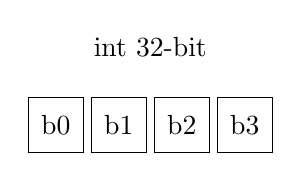
\begin{tikzpicture}[node distance=0.5cm]
    \tikzstyle{cell}=[draw, minimum width=0.7cm, minimum height=0.7cm]
    \node at (0,0) [cell] {b0};
    \node at (0.8,0) [cell] {b1};
    \node at (1.6,0) [cell] {b2};
    \node at (2.4,0) [cell] {b3};
    \node at (1.2,1) {int 32-bit};
  \end{tikzpicture}
  \caption{Contoh representasi integer 32-bit sebagai 4 byte}
\end{figure}

\section{Deklarasi \& Inisialisasi Variabel}
Deklarasi menetapkan nama, tipe, cakupan; inisialisasi awal mencegah nilai sampah (khususnya di C). C++ mendukung inisialisasi terbraket yang lebih aman, sedangkan Pascal memiliki bagian \texttt{var} yang eksplisit \parencite{pascal-tutorial-wikibooks,gnu-c-manual,cpp-reference}.

\subsection{Contoh Deklarasi dan Inisialisasi}

Program berikut menunjukkan cara mendeklarasikan variabel dengan berbagai tipe data dan menginisialisasinya dengan nilai awal:

\begin{lstlisting}[language=Pascal, caption={Deklarasi dan inisialisasi di Pascal}]
program Vars;
var
  count: integer = 0;
  ratio: double = 0.5;
  letter: char = 'A';
  flag: boolean = true;
begin
  Writeln(count, ' ', ratio:0:2, ' ', letter, ' ', flag);
end.
\end{lstlisting}

\begin{lstlisting}[language=C, caption={Deklarasi dan inisialisasi di C}]
#include <stdio.h>
int main(void) {
  int count = 0;
  double ratio = 0.5;
  char letter = 'A';
  _Bool flag = 1; // C99
  printf("%d %.2f %c %s\n", count, ratio, letter, flag?"true":"false");
  return 0;
}
\end{lstlisting}

\begin{lstlisting}[language=C++, caption={Deklarasi dan inisialisasi di C++}]
#include <iostream>
using namespace std;

int main() {
  int count{0};
  double ratio{0.5};
  char letter{'A'};
  bool flag{true};
  cout << count << ' ' << ratio << ' ' << letter << ' ' << boolalpha << flag << '\n';
}
\end{lstlisting}

Disiplin penamaan yang konsisten meningkatkan keterbacaan. Bila lingkup variabel terlalu panjang, pecahlah fungsi menjadi unit lebih kecil. Gunakan \texttt{const} (atau setara) untuk nilai yang tidak boleh berubah.

Pada C/C++, pahami durasi penyimpanan (otomatis, statik, dinamis) untuk mengelola siklus hidup. Deklarasi dekat titik penggunaan menurunkan kompleksitas. Pada Pascal, bagian \texttt{var} menjaga struktur yang mudah diaudit \parencite{free-pascal-docs,gnu-c-manual}.

\section{Input / Output Dasar}
Masukan/keluaran (I/O) memungkinkan program berinteraksi dengan pengguna dan berkas. Pascal memakai \texttt{Read/Readln} dan \texttt{Write/Writeln}; C memakai \texttt{scanf/printf}; C++ memakai stream \texttt{std::cin/std::cout} dan manipulator \texttt{<iomanip>} \parencite{w3pascal-io,gnu-c-manual,cplusplus-io,cpp-iomanip}.

\subsection{Perbandingan Sintaks I/O Dasar}
\begin{table}[H]
  \centering
  \caption{Perbandingan ringkas perintah I/O}
  \label{tab:io-basic}
  \begin{tabular}{@{}lll@{}}
    \toprule
    Bahasa & Output & Input \\
    \midrule
    Pascal & \texttt{Writeln('...')} & \texttt{Readln(x)} \\
    C      & \texttt{printf("...")} & \texttt{scanf("\%d", \&x)} \\
    C++    & \texttt{std::cout << "..."} & \texttt{std::cin >> x} \\
    \bottomrule
  \end{tabular}
\end{table}

\subsection{Contoh Input/Output Dasar}
Berikut contoh membaca dua bilangan bulat dan menampilkan hasil penjumlahannya. Perhatikan perbedaan I/O \parencite{w3pascal-io,gnu-c-manual,cpp-reference}.

Contoh pertama mendemonstrasikan cara membaca dua bilangan dari pengguna, menjumlahkannya, dan menampilkan hasilnya di Pascal:

\begin{lstlisting}[language=Pascal, caption={Menjumlah dua bilangan pada Pascal}]
program SumTwo;
var
  a, b, total: integer;
begin
  Readln(a);
  Readln(b);
  total := a + b;
  Writeln('Jumlah = ', total);
end.
\end{lstlisting}

Di C, operasi yang sama menggunakan \texttt{scanf} untuk input dan \texttt{printf} untuk output:

\begin{lstlisting}[language=C, caption={Menjumlah dua bilangan pada C}]
#include <stdio.h>

int main(void) {
  int a, b;
  scanf("%d %d", &a, &b);
  printf("Jumlah = %d\n", a + b);
  return 0;
}
\end{lstlisting}

C++ menggunakan stream operator (\texttt{cin} dan \texttt{cout}) untuk I/O yang lebih type-safe:

\begin{lstlisting}[language=C++, caption={Menjumlah dua bilangan pada C++}]
#include <iostream>
using namespace std;

int main() {
  int a, b;
  cin >> a >> b;
  cout << "Jumlah = " << (a + b) << '\n';
  return 0;
}
\end{lstlisting}

\begin{table}[H]
  \centering
  \small
  \caption{Instruksi Input/Output pada Pascal, C, dan C++}
  \begin{tabular}{@{}llll@{}}
    \toprule
    Operasi & Pascal & C & C++ \\
    \midrule
    Input standar & \texttt{Read()}, \texttt{Readln()} & \texttt{scanf()}, \texttt{fgets()} & \texttt{cin >>}, \texttt{getline()} \\
    Output standar & \texttt{Write()}, \texttt{Writeln()} & \texttt{printf()} & \texttt{cout <<} \\
    Output error & - & \texttt{fprintf(stderr)} & \texttt{cerr <<} \\
    Format output & \texttt{var:width:decimal} & \texttt{printf("\%format")} & manipulator \texttt{iomanip} \\
    Input string & \texttt{Readln(str)} & \texttt{fgets(...)} & \texttt{getline(...)} \\
    \bottomrule
  \end{tabular}
  \\\parencite{w3pascal-io,gnu-c-manual,cplusplus-io,cpp-iomanip}
\end{table}

Pisahkan keluaran kesalahan (\texttt{stderr}) dari keluaran normal untuk memudahkan otomasi. Pada C, gunakan \texttt{snprintf} untuk mencegah luapan buffer. Pada C++, gunakan \texttt{std::setw}, \texttt{std::setprecision} untuk keluaran yang rapi \parencite{gnu-c-manual,cpp-reference,cpp-iomanip}.

\subsection{Diagram Arus I/O}
\begin{figure}[H]
  \centering
  \begin{tikzpicture}[node distance=1.6cm, >=Stealth]
    \tikzstyle{box}=[rectangle, draw, rounded corners, align=center, minimum width=3.1cm, minimum height=1cm]
    \node[box] (kbd) {Keyboard/\newline Berkas Masuk};
    \node[box, right=of kbd] (prog) {Program};
    \node[box, right=of prog] (term) {Terminal/\newline Berkas Keluar};
    \draw[->] (kbd) -- node[above]{input} (prog);
    \draw[->] (prog) -- node[above]{output} (term);
  \end{tikzpicture}
  \caption{Arus I/O sederhana antara pengguna/berkas dan program}
  \label{fig:io-flow}
\end{figure}

\subsection{Contoh I/O Angka dan Pemformatan}

Program berikut menunjukkan cara memformat output angka dengan jumlah desimal tertentu dan membaca input dari pengguna:

\begin{lstlisting}[language=Pascal, caption={Baca integer dan format keluaran (Pascal)}]
program IOFmt;

var
  n: integer;
begin
  Write('Masukkan angka: ');
  Readln(n);
  Writeln('Kuadrat = ', n * n);
  Writeln('Pi ~ ', 3.14159:0:2);  // 2 digit desimal
end.
\end{lstlisting}

Di C, pemformatan output menggunakan format specifier dalam \texttt{printf}:

\begin{lstlisting}[language=C, caption={Baca integer dan format keluaran (C)}]
#include <stdio.h>
int main(void) {
  int n;
  printf("Masukkan angka: ");
  scanf("%d", &n);
  printf("Kuadrat = %d\n", n*n);
  printf("Pi ~ %.2f\n", 3.14159);
  return 0;
}
\end{lstlisting}

C++ menggunakan manipulator dari \texttt{<iomanip>} untuk mengontrol format output:

\begin{lstlisting}[language=C++, caption={Baca integer dan format keluaran (C++)}]
#include <iostream>
#include <iomanip>
using namespace std;

int main() {
  int n;
  cout << "Masukkan angka: ";
  cin >> n;
  cout << "Kuadrat = " << n*n << "\n";
  cout << fixed << setprecision(2) << "Pi ~ " << 3.14159 << "\n";
  return 0;
}
\end{lstlisting}

\subsection{Contoh I/O String (Program Interaktif)}

Program interaktif berikut membaca nama pengguna dan menampilkan salam. Ini mendemonstrasikan cara kerja I/O string dasar:

\begin{lstlisting}[language=Pascal, caption={Input nama pada Pascal}]
program Greet;

var
  name: string;
begin
  Write('Nama Anda? ');
  Readln(name);
  Writeln('Halo, ', name, '!');
end.
\end{lstlisting}

Di C, input string memerlukan array karakter dan fungsi \texttt{fgets} yang lebih aman daripada \texttt{gets}:

\begin{lstlisting}[language=C, caption={Input nama pada C}]
#include <stdio.h>
int main(void) {
  char name[64];
  printf("Nama Anda? ");
  fgets(name, sizeof name, stdin);
  printf("Halo, %s", name); // fgets menyertakan newline
  return 0;
}
\end{lstlisting}

C++ menggunakan \texttt{getline} untuk membaca string dengan spasi, berbeda dengan operator \texttt{>>} yang berhenti di whitespace:

\begin{lstlisting}[language=C++, caption={Input nama pada C++}]
#include <iostream>
using namespace std;

int main() {
  char name[64];
  cout << "Nama Anda? ";
  cin.getline(name, sizeof(name));
  cout << "Halo, " << name << "!\n";
  return 0;
}
\end{lstlisting}

\subsection{Ringkasan Pemformatan}
\begin{table}[H]
  \centering
  \caption{Ringkasan pemformatan angka}
  \begin{tabular}{@{}lll@{}}
    \toprule
    Bahasa & Contoh & Keterangan \\
    \midrule
    Pascal & \texttt{real:0:2} & 2 digit desimal \\
    C & \texttt{"\textbackslash\%.2f"} & 2 digit desimal (\texttt{printf}) \\
    C++ & \texttt{std::fixed}, \texttt{std::setprecision(2)} & 2 digit desimal \\
    \bottomrule
  \end{tabular}
  \\\parencite{w3pascal-io,gnu-c-manual,cpp-iomanip}
\end{table}

\subsection{Cheat Sheet Format String (C)}
\begin{table}[H]
  \centering
  \caption{Specifier umum untuk \texttt{printf}/\texttt{scanf} (ringkas)}
  \small
  \begin{tabular}{@{}llll@{}}
    \toprule
    Nilai & \texttt{printf} & \texttt{scanf} & Catatan \\
    \midrule
    \texttt{int} & \texttt{\%d} & \texttt{\%d} & basis desimal \\
    \texttt{long} & \texttt{\%ld} & \texttt{\%ld} & \texttt{l} untuk long \\
    \texttt{long long} & \texttt{\%lld} & \texttt{\%lld} & \texttt{ll} untuk long long \\
    \texttt{unsigned} & \texttt{\%u} & \texttt{\%u} & tanpa tanda \\
    \texttt{double} & \texttt{\%f} & \texttt{\%lf} & beda antara printf dan scanf \\
    \texttt{char} & \texttt{\%c} & \texttt{\%c} & satu karakter \\
    string C & \texttt{\%s} & \texttt{\%s} & hati-hati overflow (batasi lebar) \\
    pointer & \texttt{\%p} & - & tampilkan alamat \\
    \bottomrule
  \end{tabular}
  \\\parencite{c-printf,c-scanf}
\end{table}

\paragraph{Tips.} Pada \texttt{scanf}, tambahkan lebar maksimum: \texttt{"\%63s"} untuk buffer 64 byte. Periksa nilai kembalian untuk memastikan jumlah item yang berhasil diparse benar.

\subsection{Sinkronisasi I/O C++ dan Kinerja}
Secara bawaan, \texttt{iostream} disinkronkan dengan stdio untuk kompatibilitas. Untuk kinerja lebih baik pada input besar, dapat dinonaktifkan sinkronisasi dengan \texttt{ios::sync\_\allowbreak{}with\_\allowbreak{}stdio(false)} dan \texttt{cin.tie(nullptr)}. Namun, hindari mencampur pemanggilan stdio dan iostream. Lihat \parencite{cpp-sync-with-stdio} untuk detail teknis.

\section{Rangkuman Materi}
\begin{itemize}
  \item Tipe data dasar lintas bahasa dan model data 64-bit (LP64 vs LLP64).
  \item Tipe tetap-lebar \texttt{<stdint.h>/<cstdint>} dan batas nilai melalui \texttt{numeric\_limits}.
  \item Deklarasi dan inisialisasi variabel; perbedaan format I/O di Pascal, C, C++.
  \item Tabel ringkas specifier C, contoh parsing numerik yang tangguh, dan sinkronisasi I/O C++.
  \item Diagram memori 32-bit, tips casting aman, dan kiat pemecahan masalah umum.
\end{itemize}
\end{document}
